\section{Nutrient Transport}
In order to build new cellular mass, the molecular and elemental building blocks
must be scavenged from the environment in different forms. Carbon, for example,
is acquired via the transport of carbohydrates and sugar alcohols with some
carbon sources receiving preferential treatment in their consumption
\citep{monod1947}. Phosphorus, sulfur, and nitrogen, on the other hand, are
harvested primarily in the forms of inorganic salts, namely phosphate, sulfate,
and ammonia \citep{jun2018, assentoft2016, stasi2019, antonenko1997,
rosenberg1977, willsky1973}. All of these compounds have different
permeabilities across the cell membrane and most require some energetic
investment either via ATP hydrolysis or through the proton electrochemical
gradient to bring the material across the hydrophobic cell membrane. Given the
diversity of biological transport mechanisms and the vast number of inputs
needed to build a cell, we begin by considering transport of elemental
requirements as a possible rate-limiting step of bacterial cell division.


The elemental composition of \textit{E. coli} has received much quantitative
attention over the past half century \citep{neidhardt1991, taymaz-nikerel2010,
heldal1985, bauer1976}, providing us with a starting point for estimating the
copy numbers of various transporters. While there is some variability in the
exact elemental percentages (with different uncertainties), we can estimate that
the dry mass of a typical \textit{E. coli} cell is $\approx$ 45\% carbon (BNID:
100649, \cite{milo2010}), $\approx$ 15\% nitrogen (BNID: 106666,
\cite{milo2010}), $\approx$ 3\% phosphorus (BNID: 100653, \cite{milo2010}), and
1\% sulfur (BNID: 100655, \cite{milo2010}). In the coming paragraphs, we will
examine how many transporters and/or channels must be present to maintain these
elemental compositions with a moderate doubling time of 6,000 s.

\subsection{Carbon Transport}
We begin with the most abundant element by mass, carbon. Using $\approx$ 0.3
pg as the typical \textit{E. coli} dry mass (BNID: 103904, \cite{milo2010}),
we estimate that $\approx 10^{10}$ carbon atoms must be brought into the cell
in order to double all of the carbon-containing molecules
(\FIG{carbon_tport}(A, top))). Typical laboratory growth conditions, such as
those explored in the aforementioned proteomic data sets, provide carbon as
single class of sugar such as glucose, galactose, or xylose to name a few.
\textit{E. coli} has evolved myriad mechanisms by which these sugars can be
transported across the cell membrane. One such mechanism of transport is via
the PTS system which is a highly modular system capable of transporting a
diverse range of sugars \citep{escalante2012}. The glucose-specific component
of this system transports $\approx$ 200 glucose molecules per second per
channel (BNID: 114686, \cite{milo2010}). Making the assumption that this is a
typical sugar transport rate, coupled with the need to transport 10$^{10}$
carbon atoms, we arrive at the conclusion that on the order of 1,000
transporters must be expressed in order to bring in enough carbon atoms to
divide in 6,000 s, diagrammed in the top panel of \FIG{carbon_tport}(A). This
estimate, along with the observed average number of carbohydrate transporters
present in the proteomic data sets \citep{schmidt2016,
peebo2015,valgepea2013,li2014}, is shown in \FIG{carbon_tport}(A). While we
estimate 1,000 transporters are needed, the data reveals that at a division
time of $\approx 6,000$ s there is nearly a ten-fold excess of transporters.
Furthermore, the data illustrates that the average number of carbohydrate
transporters present is largely-growth rate independent.

\begin{figure}
    \begin{fullwidth}
    \centering{
    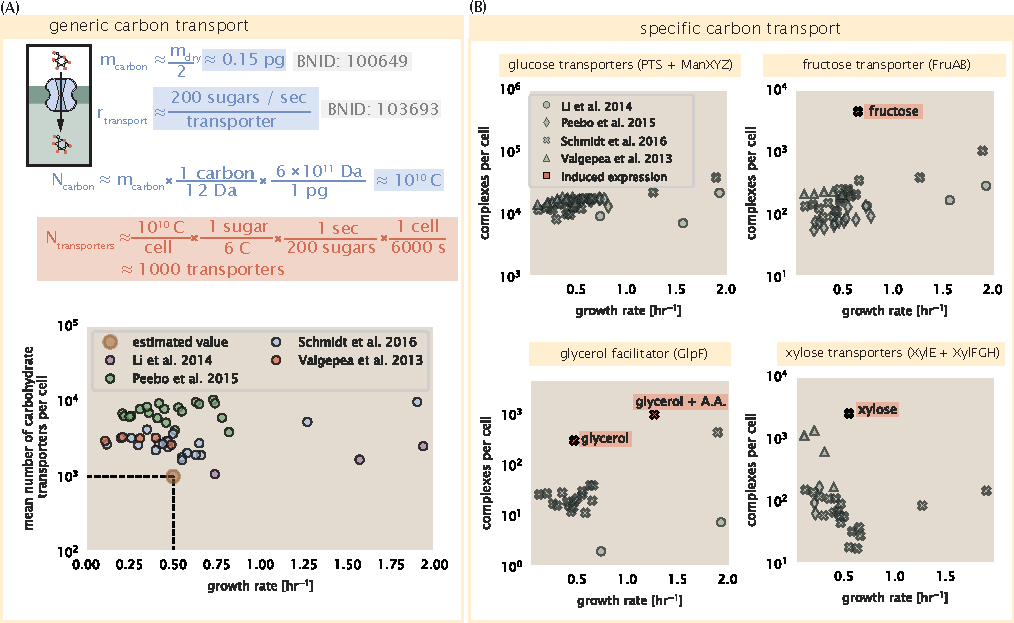
\includegraphics{main_figs/fig2_carbon_transport.pdf}
    \caption{\textbf{The abundance of carbon transport systems across growth
    rates.} (A) A simple estimate for the minimum number of generic carbohydrate
    transport systems (top) assumes $\approx 10^{10}$ C are needed to complete
    division, each transported sugar contains $\approx 6$ C, and each
    transporter conducts sugar molecules at a rate of $\approx 200$ per second.
    Bottom plot shows the estimated number of transporters needed at a growth
    rate of $\approx 0.5 $ per hr (light-brown point and dashed lines). Colored
    points correspond to the mean number of carbohydrate transporters for
    different growth conditions across different published datasets. (B) The
    abundance of various specific carbon transport systems plotted as a function
    of the population growth rate. Red points and red-highlighted text indicate conditions in which the
    only source of carbon in the growth medium induces expression of the
    transport system.}
    \label{fig:carbon_tport}
    }
    \end{fullwidth}
\end{figure}

The estimate presented in \FIG{carbon_tport}(A) neglects any specifics of the
regulation of carbon transport system and presents a data-averaged view of how
many carbohydrate transporters are present on average. Using the diverse array
of growth conditions explored in the proteomic data sets, we can explore how
individual carbon transport systems depend on the population growth rate. In
\FIG{carbon_tport}(B), we show the total number of carbohydrate transporters
specific to different carbon sources. A striking observation, shown in the
top-left plot of \FIG{carbon_tport}(B), is the constancy in the expression of the
glucose-specific transport systems (the PtsG enzyme of the PTS system and the
glucose-transporting ManXYZ complex). Additionally, we note that the total number
of glucose-specific transporters is tightly distributed $\approx 10^4$ per cell,
an order of magnitude beyond the estimate shown in \FIG{carbon_tport}(A). This
illustrates that \textit{E. coli} maintains a substantial number of complexes
present for transporting glucose which is known to be the preferential carbon
source \citep{monod1947, liu2005a, aidelberg2014}.

It is now understood that a large number of metabolic operons are regulated
with dual-input logic gates that are only expressed when glucose
concentrations are low (mediated by cyclic-AMP receptor protein CRP) and the
concentration of other carbon sources are elevated \citep{gama-castro2016, zhang2014a}. A
famed example of such dual-input regulatory logic is in the regulation of the
\textit{lac} operon which is only natively activated in the absence of glucose and the
presence of allolactose, an intermediate in lactose metabolism \citep{jacob1961}, though
we now know of many other such examples \citep{ireland2020, gama-castro2016,
belliveau2018}. This illustrates that once glucose is depleted from the
environment, cells have a means to dramatically increase the abundance of the
specific transporter needed to digest the next sugar that is present. Several
examples of induced expression of a specific carbon-source transporters are
shown in \FIG{carbon_tport}(B). Points colored in red (labeled by red
text-boxes) correspond to growth conditions in which the specific carbon source
(glycerol, xylose, or fructose) is present. These plots show that, in the
absence of the particular carbon source, expression of the transporters is
maintained on the order of $\sim 10^2$ per cell. However, when induced, the
transporters become highly-expressed and are present on the order of $\sim
10^4$ per cell, which exceeds the generic estimate given in
\FIG{carbon_tport}(A). Together, this generic estimation and the specific
examples of induced expression suggest that transport of carbon across the cell
membrane, while critical for growth, is not the rate-limiting step of cell division.

In the context of speeding up growth, one additional limitation  is the fact
that the cell's inner membrane is occupied by a multitude of other required
membrane proteins. Considering a rule-of-thumb for the surface area of
\textit{E. coli} of about 6 $\mu m^2$ (BNID: 101792, \cite{milo2010}), we expect
an areal density for 1,000 transporters to be approximately 200
transporters/$\mu m^2$. For a glucose transporter occupying about 50
nm$^2$/dimer, this amounts to about only 1 percent of the total inner membrane
\citep{szenk2017}. In addition, bacterial cell membranes typically have
densities of 10$^5$ proteins//$\mu m^2$ \citep{phillips2018}, implying that the
cell could accommodate more transporters if it were rate limiting.

\subsection{Phosphorus and Sulfur Transport}
We now turn our attention towards other essential elements, namely phosphorus and
sulfur. Phosphorus is critical to the cellular energy economy in the form of
high-energy phosphodiester bonds making up DNA, RNA, and the NTP energy pool as
well as playing a critical role in the post-translational modification of
proteins and defining the polar-heads of lipids. In total, phosphorus
makes up $\approx$3\% of the cellular dry mass which in typical experimental conditions is in the form of inorganic phosphate. The cell membrane
has remarkably low permeability to this highly-charged and critical molecule,
therefore requiring the expression of active transport systems. In \textit{E. coli}, the proton
electrochemical gradient across the inner membrane is leveraged to transport
inorganic phosphate into the cell \citep{rosenberg1977}.
Proton-solute symporters are widespread in \textit{E. coli} \citep{ramos1977,
booth1979} and can have rapid transport rates of 50 molecules per second for
sugars and other solutes (BNID: 103159; 111777, \cite{milo2010}). In \textit{E.
coli} the PitA phosphate transport system has been shown to very tightly coupled
with the proton electrochemical gradient with a 1:1 proton:phosphate
stoichiometric ratio \citep{harris2001, feist2007}. Illustrated in
\FIG{phospho_sulfo_tport}(A), we can estimate that $\approx$ 300
phosphate transporters are necessary to maintain an $\approx$ 3\% dry mass with
a 6,000 s division time. This estimate is again satisfied when we examine the
observed copy numbers of PitA in proteomic data sets (plot in
\FIG{phospho_sulfo_tport}(A)). While our estimate is very much in line with the
observed numbers, we emphasize that this is likely a slight over estimate of the
number of transporters needed as there are other phosphorous scavenging systems,
such as the ATP-dependent phosphate transporter Pst system which we have neglected.

Satisfied that there are a sufficient number of phosphate transporters
present in the cell, we now turn sulfur transport as another potentially rate
limiting process. Similar to phosphate, sulfate is  highly-charged
and not particularly membrane permeable, requiring active
transport. While there exists a H+/sulfate symporter in \textit{E.
coli}, it is in relatively low abundance and is not well characterized
\citep{zhang2014}. Sulfate is predominantly acquired via the ATP-dependent ABC
transporter CysUWA system which also plays an important role in selenium
transport \citep{sekowska2000, sirko1995}. While specific kinetic details of
this transport system are not readily available, generic ATP transport
systems in prokaryotes are on the order of 1 to 10 molecules per second
(BNID: 109035, \cite{milo2010}). Combining this generic
transport rate, measurement of sulfur comprising 1\% of dry mass, and a 6,000
second division time yields an estimate of $\approx$ 1000 CysUWA
complexes per cell (\FIG{phospho_sulfo_tport}(B)). Once again, this estimate
is in notable agreement with proteomic data sets, suggesting that there are
sufficient transporters present to acquire the necessary sulfur. In a similar
spirit of our estimate of phosphorus transport, we emphasize that this is
likely an overestimate of the number of necessary transporters as we have
neglected other sulfur scavenging systems that are in lower
abundance.


\begin{figure*}
    \begin{fullwidth}
    \centering{
        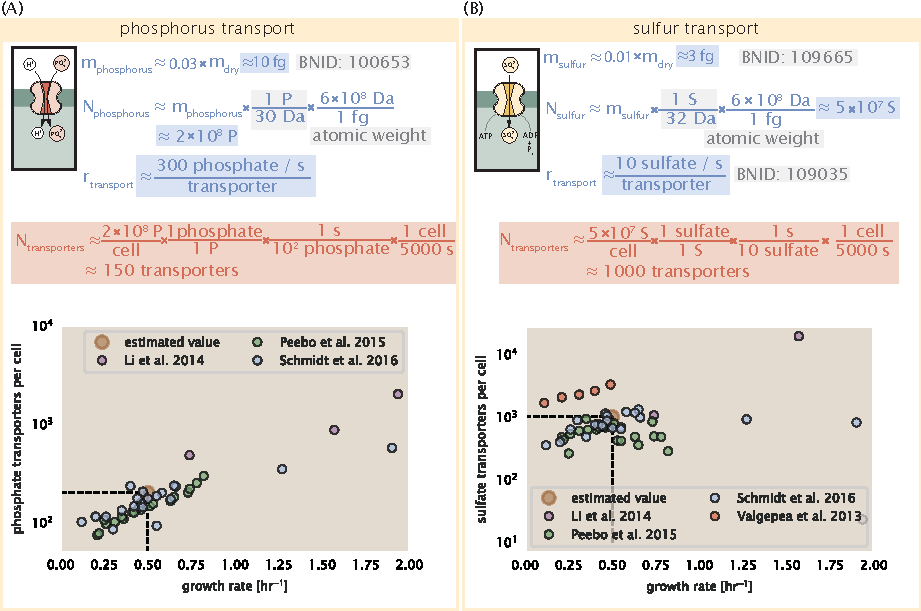
\includegraphics{main_figs/fig3_phospho_sulfo_transport.pdf}
        \caption{\textbf{Estimates and measurements of phosphate and sulfate
        transport systems as a function of growth rate.} (A) Estimate for the
        number of PitA phosphate transport systems needed to maintain a 3\%
        phosphorus \textit{E. coli} dry mass. Points in plot correspond to the
        the total number of PitA transporters per cell. (B) Estimate of the
        number of CysUWA complexes necessary to maintain a 1\% sulfur \textit{E.
        coli} dry mass. Points in plot correspond to average number of CysUWA
        transporter complexes that can be formed given the transporter
        stoichiometry [CysA]$_2$[CysU][CysW][Sbp/CysP].}
        \label{fig:phospho_sulfo_tport}
    }
    \end{fullwidth}
\end{figure*}

\subsection{Nitrogen Transport}
Finally, we turn to nitrogen transport as the last remaining transport system
highlighted in \FIG{categories}. Unlike phosphate, sulfate, and various sugar
molecules, nitrogen in the form of ammonia can readily diffuse across the
cell membrane and has a permeability on par with water ($\approx 10^5$ nm/s,
BNID:110824 \cite{milo2010}). In particularly nitrogen-poor
conditions, \textit{E. coli} expresses a transporter (AmtB) which appears to aid in
nitrogen assimilation, though the mechanism and kinetic details of transport
is still a matter of debate \citep{heeswijk2013a, khademi2004}. Beyond ammonia,
another plentiful source of nitrogen come in the form of glutamate, which has it's
own complex metabolism and scavenging pathways. However, nitrogen is plentiful
in the growth conditions examined in this work, permitting us to neglect
nitrogen transport as a potential rate limiting process in cell division.
